\section{Opgave 5}

Vi har hentet et lydklip af en DTMF telefon hvor taste styk giver forskellige lyde alt efter hvad for en tast man tyrkker på, DFT plottet og det udglattede plot ses i figur  \autoref{fig:telephone_dial_up}.


\begin{figure}[H]
\centering
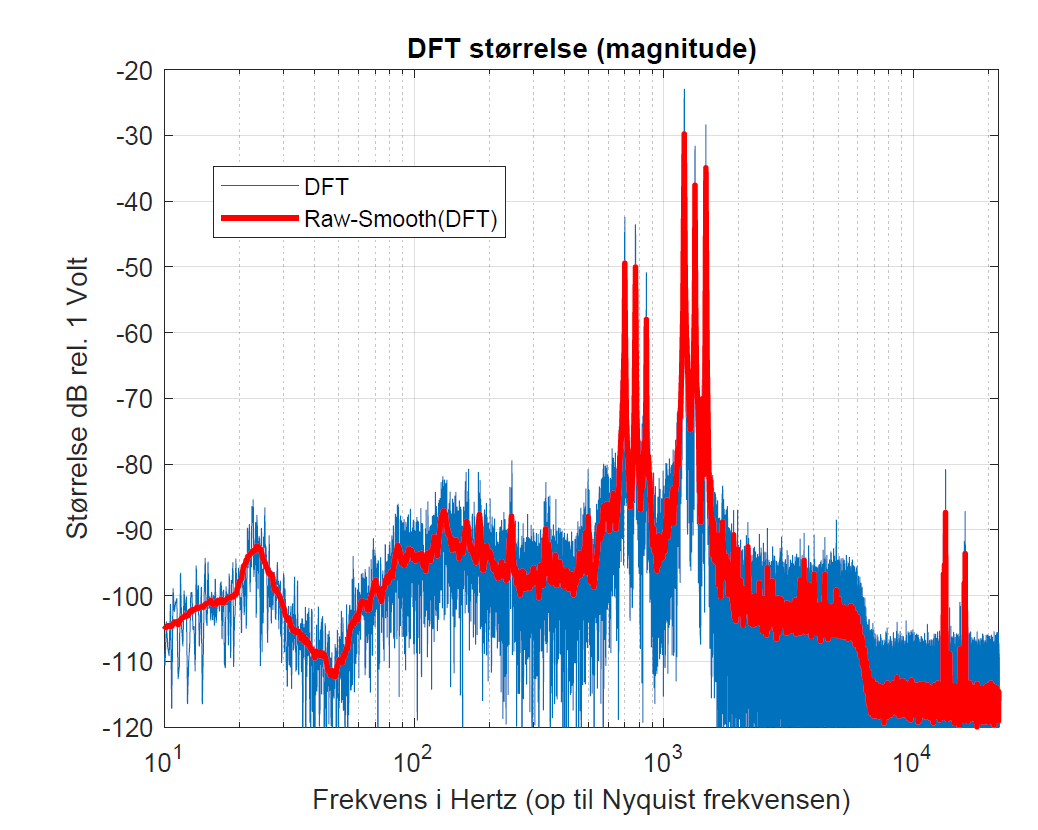
\includegraphics[width=\textwidth]{"figures/opgave5_1.png"}
\caption{DFT i blå og et udglatning (raw smooth) af DFT i rød}
\label{fig:telephone_dial_up}
\end{figure}

Hertil har vi googlet os frem til at DTFM lyd tonerne er lavet ud af en blanding af to fundamentale toner, på figur \autoref{fig:DTFM_blandning} ses blandings matricen for DTFM toner. 

\begin{figure}[H]
\centering
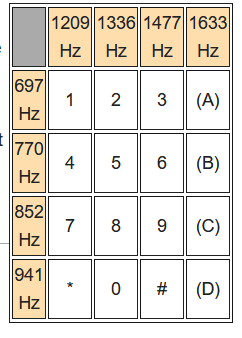
\includegraphics[width=0.3\textwidth]{"figures/DTFM.png"}
\caption{Blandings matricen for DTMF toner (kilde:https://da.wikipedia.org/wiki/DTMF)}
\label{fig:DTFM_blandning}
\end{figure}

Vi kan nu indetifiser de 6 fundamentale toner i telefon lydklippet. På figur \autoref{fig:telephone_dial_up_zoom} ses det område på DFT plottet hvor de 6 fundamentale toner er fundet. 

\begin{figure}[H]
\centering
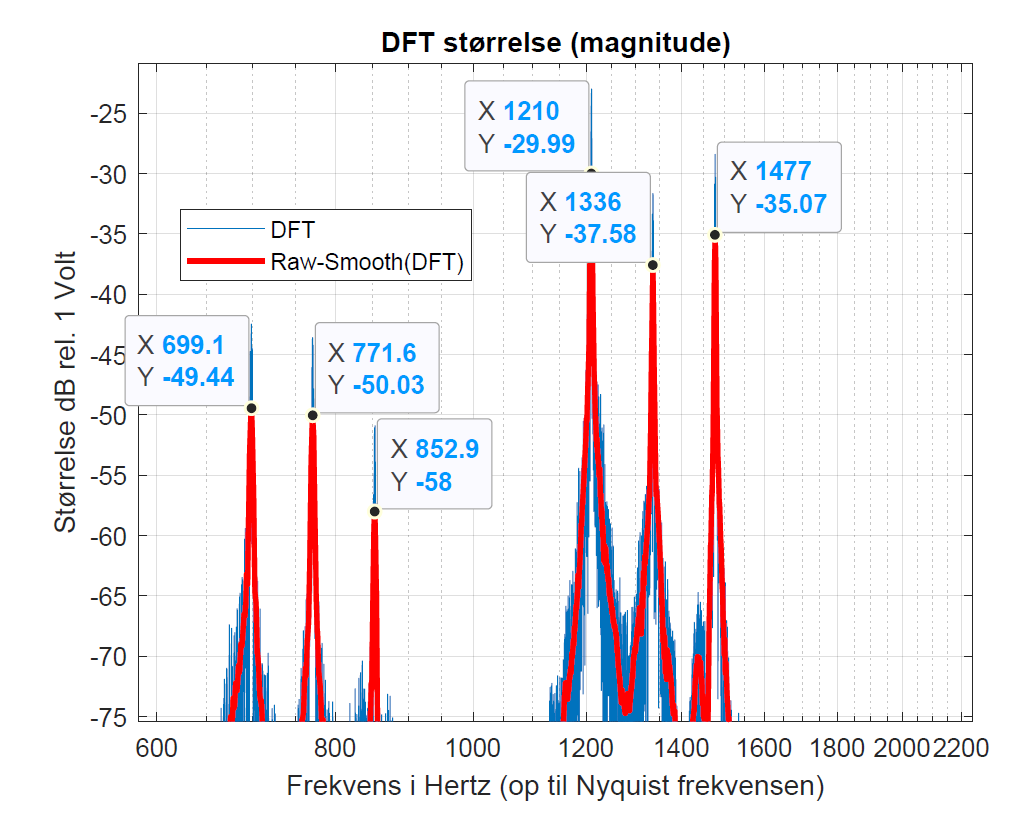
\includegraphics[width=\textwidth]{"figures/opgave5_zoom_1.png"}
\caption{Zoom af det specifikke område hvor de 6 fundamentale DTMF blandings toner er identifiseret. DFT i blå og et udglatning (raw-smooth) af DFT i rød}
\label{fig:telephone_dial_up_zoom}
\end{figure}

Vi aflæser at de 6 peaks på figur \autoref{fig:telephone_dial_up_zoom} svare til føglende frekvenser: ca. 699 , 771, 852, 1210, 1336, 1477. 
Dette passer meget godt med de angivede fundamentale blandinsfrekvenser. 

\section{Opgave 6}

Her undersøger vi tre forskellige lydklip, vinglas knipset, kompressor og musik klip. 

\begin{figure}[H]
\centering
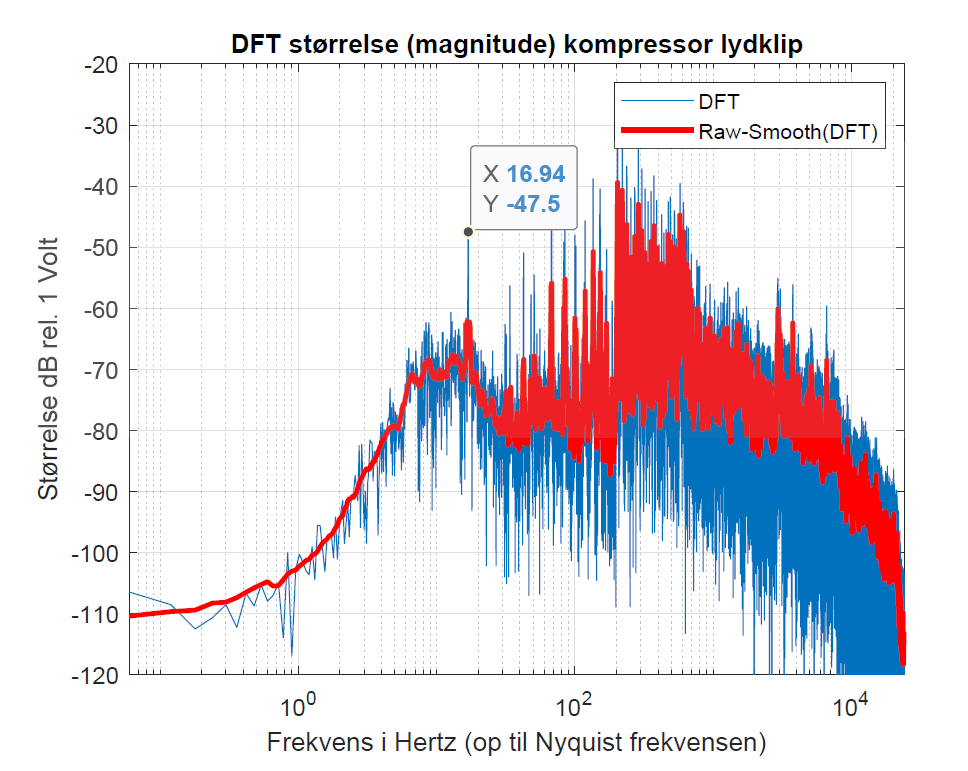
\includegraphics[width=\textwidth]{"figures/opgave6_kom_1.png"}
\caption{DFT i blå og et udglatning (raw smooth) af DFT i rød, hvor kompressor pumpen hadstigheden på 16Hz}
\label{fig:kompressor}
\end{figure}

\begin{figure}[H]
\centering
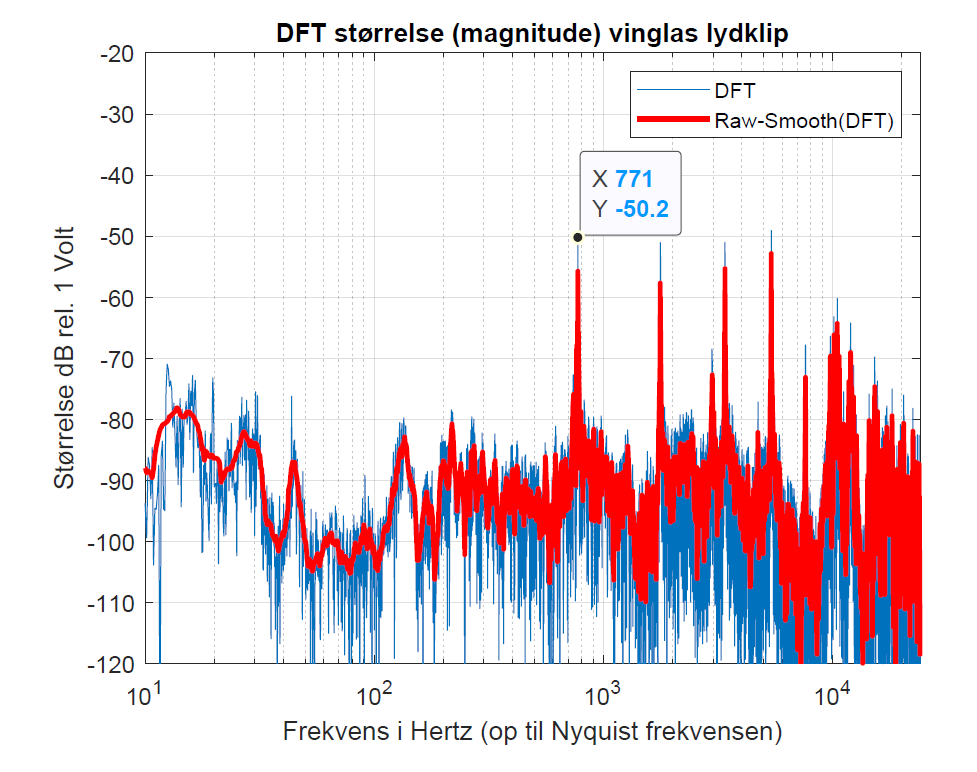
\includegraphics[width=\textwidth]{"figures/opgave6_vinglas_1.png"}
\caption{DFT i blå og et udglatning (raw smooth) af DFT i rød, hvor vinglas egenfrekvensen på 771Hz}
\label{fig:vinglas}
\end{figure}

\begin{figure}[H]
\centering
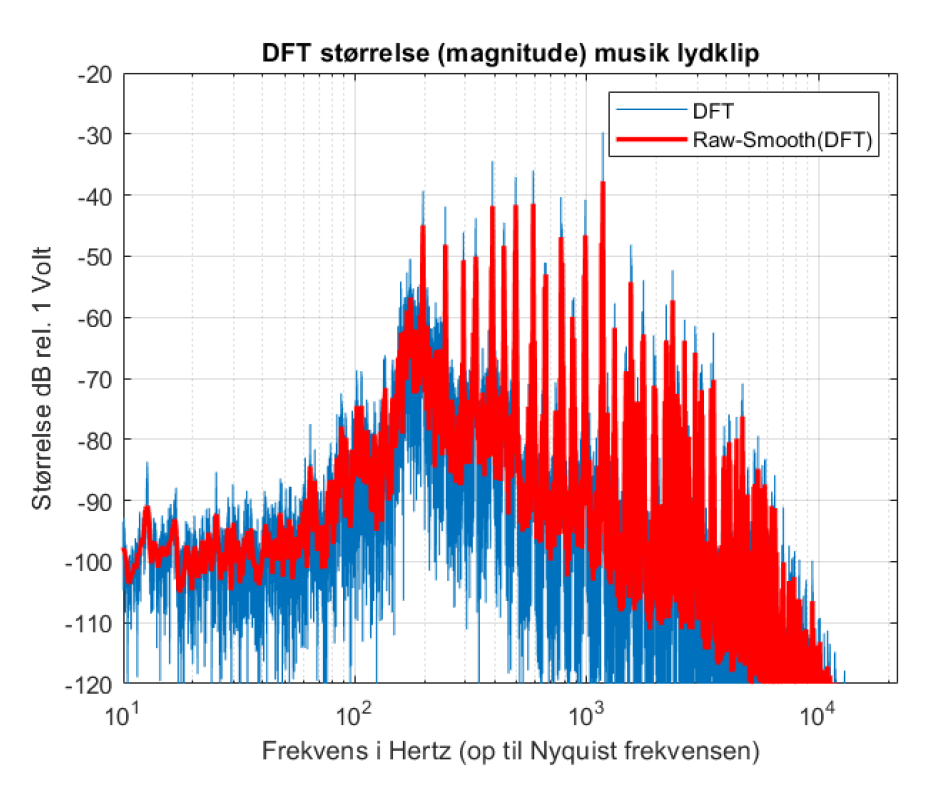
\includegraphics[width=\textwidth]{"figures/opgave6_musik_1.png"}
\caption{DFT i blå og et udglatning (raw smooth) af DFT i rød}
\label{fig:musik}
\end{figure}